\documentclass{article}

\usepackage{amsmath,amssymb,graphicx,geometry,enumitem}
\usepackage{xepersian}

\newcounter{qnumber}
\setcounter{qnumber}{1}

\newcommand{\Q}{
\textbf{سوال \theqnumber)}
\stepcounter{qnumber}
}

\setlength{\parindent}{0mm}
\setlength{\parskip}{3mm}
\settextfont{XB Niloofar}

\begin{document}

\begin{center}
\Large

به نام او

آزمون میان ترم سیگنال ها و سیستم ها
\end{center}

\hrulefill

\large

\Q
با بیان دلایل کافی، بررسی کنید هر یک از سیستم های پیوسته‌ی زیر، کدام ویژگی های علی بودن، خطی بودن، پایدار بودن، مستقل از زمان بودن و معکوس پذیری را دارا هستند (در هر یک از این سیستمها، $x(t)$ ورودی و $y(t)$ خروجی سیستم است).

الف) 
$
y(t)=x(\cos t)
$

ب) 
$
y(t)=\frac{x(t)}{x^2(t)-t}
$

پ)
$
y(t)=\begin{cases}
x^2(t)&,\quad x(t)<0\\
x(1+t)+x(-t)&,\quad x(t)\ge 0
\end{cases}
$

ت)
$
y(t)=\begin{cases}
x(t^2)+x(-t-4)&,\quad t<0\\
x(t^3)&,\quad t\ge 0
\end{cases}
$

\Q

اگر سیگنال $x(t)$ به شکل زیر باشد و تبدیل فوریه آن را با 
$
X(j\omega)
$
نشان دهیم، بدون محاسبه مستقیم $X(j\omega)$ موارد زیر را بیابید.

الف)
$X(j0)$

ب)
$\int_{-\infty}^\infty X(j\omega) \frac{\sin \omega}{\omega} e^{j\omega}d\omega$

\begin{figure}[h]
\centering
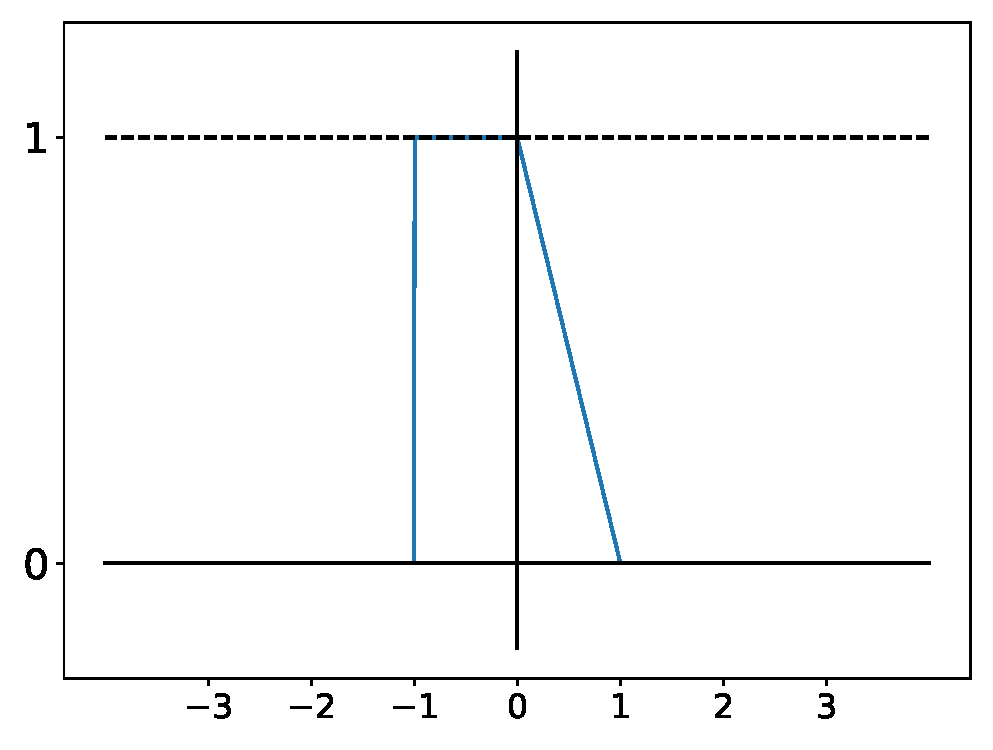
\includegraphics[width=80mm]{x11(t)}
\end{figure}

\Q

به یک سیستم LTI با تابع انتقال 
$$
H(j\omega)=\begin{cases}
2-\frac{|\omega|}{2}&,\quad |\omega|<4\\
0&,\quad \text{سایر جاها}
\end{cases}
،
$$
ورودی متناوب $x(t)$ مطابق شکل زیر داده می‌شود. خروجی این سیستم را بیابید.
\begin{figure}[h]
\centering
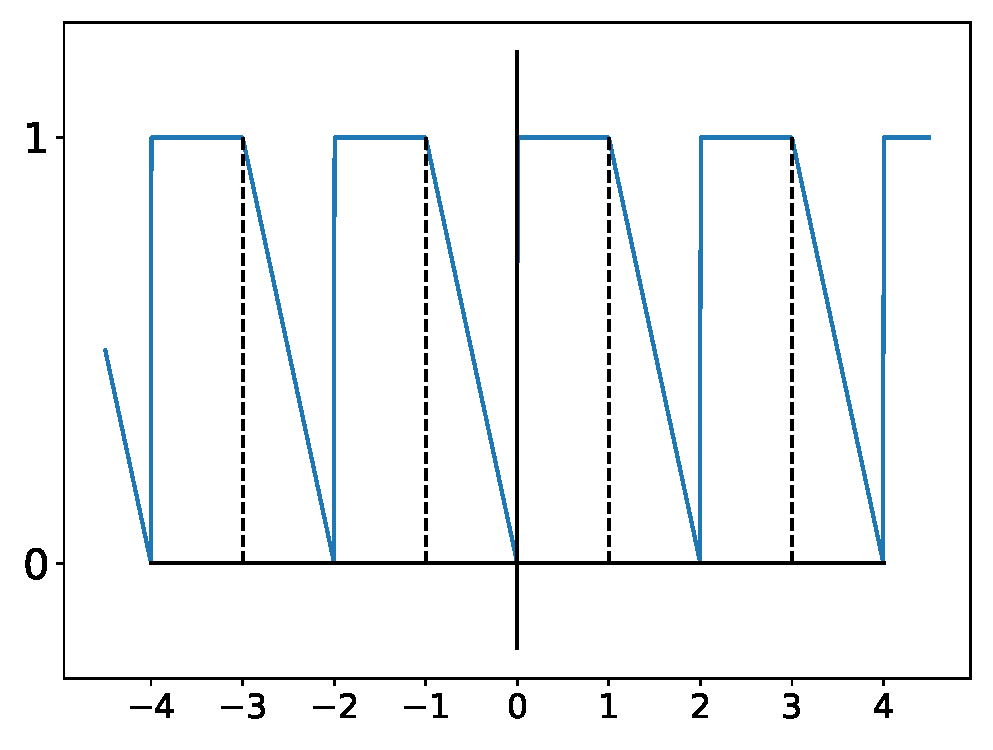
\includegraphics[width=75mm]{x1(t)}
\end{figure}

\Q
پاسخ یک سیستم LTI به ورودی 
$
x(t)=e^{-4t}u(t-2)
$
برابر 
$
y(t)
$
و پاسخ آن به ورودی 
$
\frac{dx(t)}{dt}
$
برابر 
$
-4y(t)+\frac{1}{1+t^2}
$
است. پاسخ ضربه این سیستم را بیابید.

\Q
اطلاعات زیر در مورد یک سیستم زمان-پیوسته‌ی LTI داده شده است:

\begin{enumerate}
\item
پاسخ ضربه سیستم، $h(t)$، حقیقی است.
\item
تبدیل لاپلاس سیستم دارای دو قطب و یک صفر بوده که یک قطب آن در $s=-1-2j$ است.
\item
پاسخ این سیستم به ورودی 
$
x(t)=e^t
$
برابر صفر است.
\item
$\int_{-\infty}^\infty h(t)dt=-\frac{1}{5}$
\end{enumerate}

پاسخ ضربه این سیستم را بیابید.

\Q
به سیستمی با پاسخ ضربه 
$
h(t)=\delta(t)+e^{-t}u(t)
$،
ورودی $x(t)$ با تبدیل لاپلاس 
$
X(s)=\frac{1}{(s+2)s^2}
$
و ناحیه همگرایی
$
\{s: -2<\Re\{s\}<0\}
$
داده می شود. در این صورت، خروجی این سیستم را در حوزه زمان بیابید ($\Re\{\cdot\}$ قسمت حقیقی عدد مختلط را نشان می دهد).
\end{document}